\documentclass[11pt]{report}
\usepackage{eso-pic,graphicx}
\usepackage[export]{adjustbox}
\usepackage{url}
\usepackage[top=2cm, bottom=2cm, outer=2cm, inner=2cm]{geometry}
\begin{document}
\AddToShipoutPictureBG*{
\includegraphics[width=\paperwidth,height=\paperheight]{images/bkgrnd}}
\begin{center}
\vspace*{2cm}
\textsf{\begin{Huge}
\textbf{ELP­718 ­ Telecom Software Laboratory \\
1st Semester, 2016-18 \\
Abhishek Mishra\\
27 Sep 2016, 5pm\\
Assignment-9}\\
\end{Huge}}
\vspace*{6cm}

\includegraphics[scale=0.12, center]{images/iitlogo}
\end{center}
\pagebreak
\tableofcontents
\vspace{5cm}
\pagebreak
\section{Introduction}
\vspace*{1cm}
This assignment aims to provide a better understanding of the following topics:\\

\begin{flushleft}
1. \textbf{Python}\\
Python is a widely used high-level, general-purpose, interpreted, dynamic programming language.[24][25] Its design philosophy emphasizes code readability, and its syntax allows programmers to express concepts in fewer lines of code than possible in languages such as C++ or Java.[26][27] The language provides constructs intended to enable writing clear programs on both a small and large scale.[28]

Python supports multiple programming paradigms, including object-oriented, imperative and functional programming or procedural styles. It features a dynamic type system and automatic memory management and has a large and comprehensive standard library.[29]

Python interpreters are available for many operating systems, allowing Python code to run on a wide variety of systems. Using third-party tools, such as Py2exe or Pyinstaller,[30] Python code can be packaged into stand-alone executable programs for some of the most popular operating systems, so Python-based software can be distributed to, and used on, those environments with no need to install a Python interpreter.

CPython, the reference implementation of Python, is free and open-source software and has a community-based development model, as do nearly all of its variant implementations. CPython is managed by the non-profit Python Software Foundation.
\end{flushleft}

\begin{flushleft}
2. \textbf{SQL}\\
MySQL is an open-source relational database management system (RDBMS). Its name is a combination of "My", the name of co-founder Michael Widenius' daughter,and , the abbreviation for Structured Query Language. The MySQL development project has made its source code available under the terms of the GNU General Public License, as well as under a variety of proprietary agreements. MySQL was owned and sponsored by a single for-profit firm, the Swedish company MySQL AB, now owned by Oracle Corporation. For proprietary use, several paid editions are available, and offer additional functionality.

MySQL is a central component of the LAMP open-source web application software stack (and other "AMP" stacks). LAMP is an acronym for "Linux, Apache, MySQL, Perl/PHP/Python". Applications that use the MySQL database include: TYPO3, MODx, Joomla, WordPress, phpBB, MyBB, and Drupal. MySQL is also used in many high-profile, large-scale websites, including Google (though not for searches), Facebook, Twitter, Flickr, and YouTube.

\end{flushleft}
\newpage
\section{Problem Statement 1}
	This problem requires us to take input through command line argument from the user and then process it similar to following outputs:\\
	\begin{figure}[h!]
	\centering
	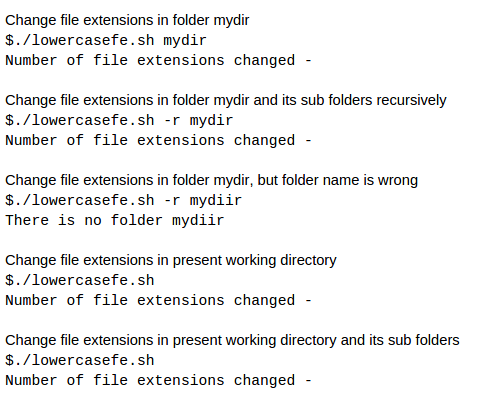
\includegraphics[scale=0.7]{images/Selection_003}	
	\end{figure}
	\subsection{Assumptions}
	The user shall input either no name to a directory or he will enter an existing directory.
	\pagebreak
	\subsection{Structure Chart and Implementation}
	\begin{figure}[h!]
	\centering
	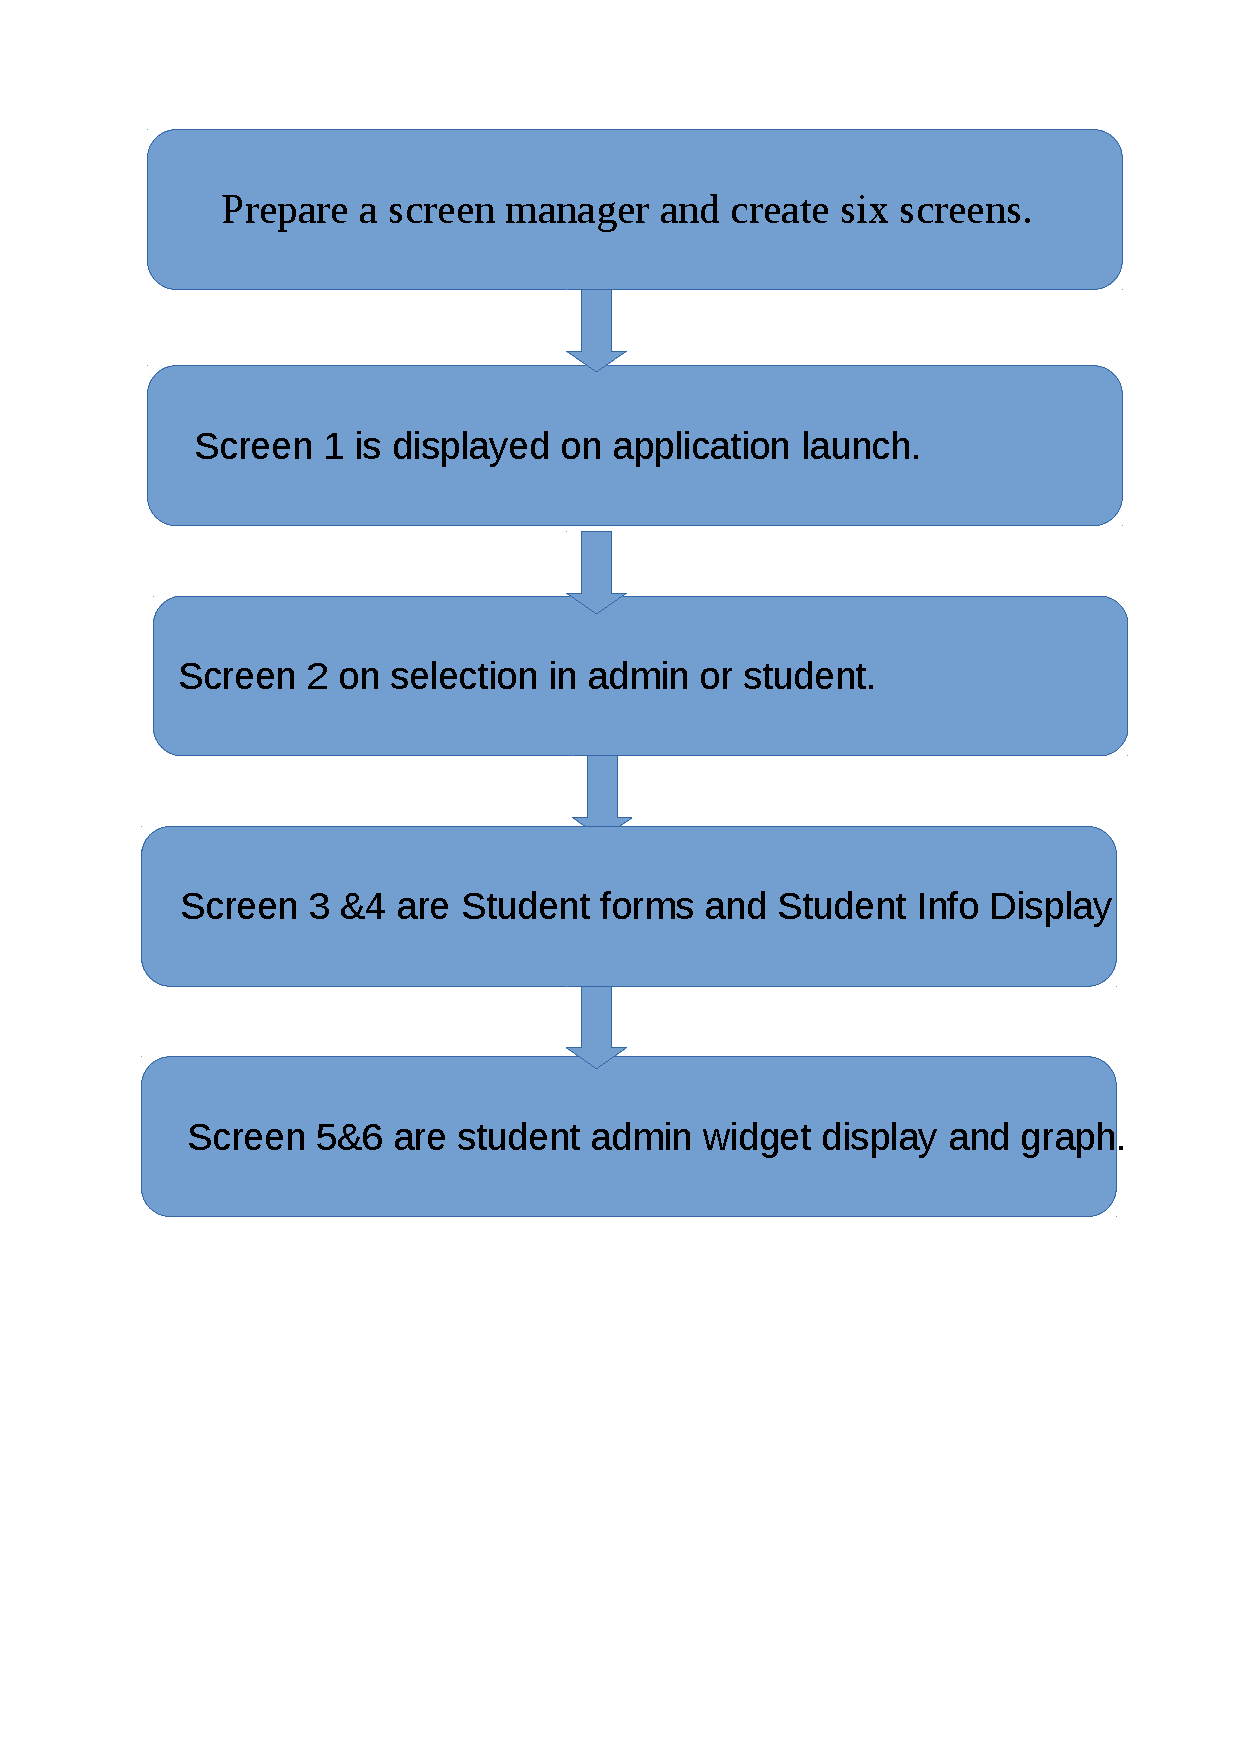
\includegraphics[scale=0.7]{images/shots11}
	\caption{Structure chart for problem 1}
	\end{figure}		
	\pagebreak
	\subsection{Screenshots}
	\begin{figure}[h!]
	\centering
	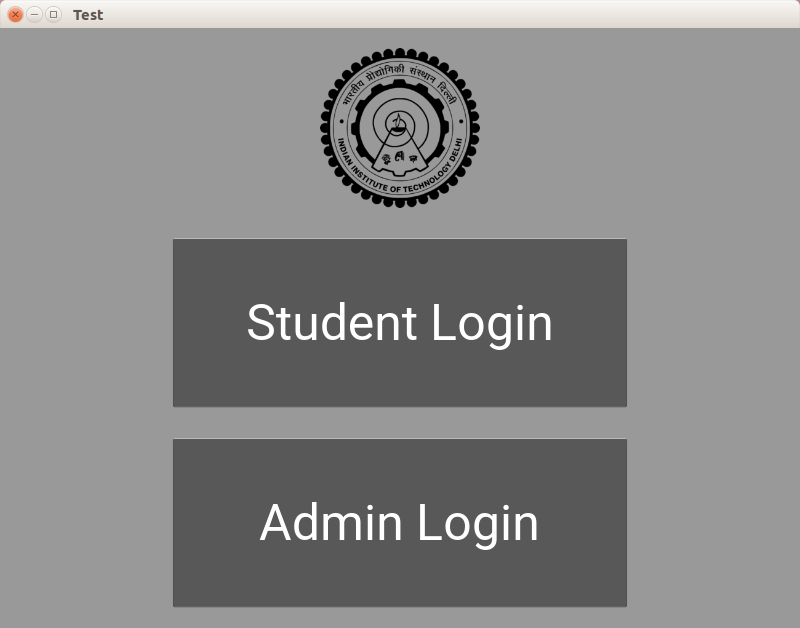
\includegraphics[scale=0.8, center]{images/screenshot1}
	\caption{Screenshot for problem statement 1}
	\end{figure}
	\pagebreak
\section{Problem Statement 2}
	The problem requires you to display system information in the following manner. \\
	\begin{figure}[h!]
	\centering
	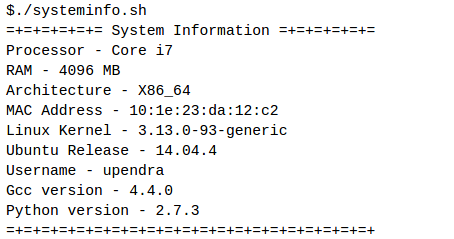
\includegraphics[scale=0.7]{images/Selection_001}	
	\end{figure}
	\subsection{Assumptions}
	The output is to be processed in the exact manner as shown in the image
	\pagebreak
	\subsection{Structure Chart}
	\begin{figure}[h!]
	\centering
	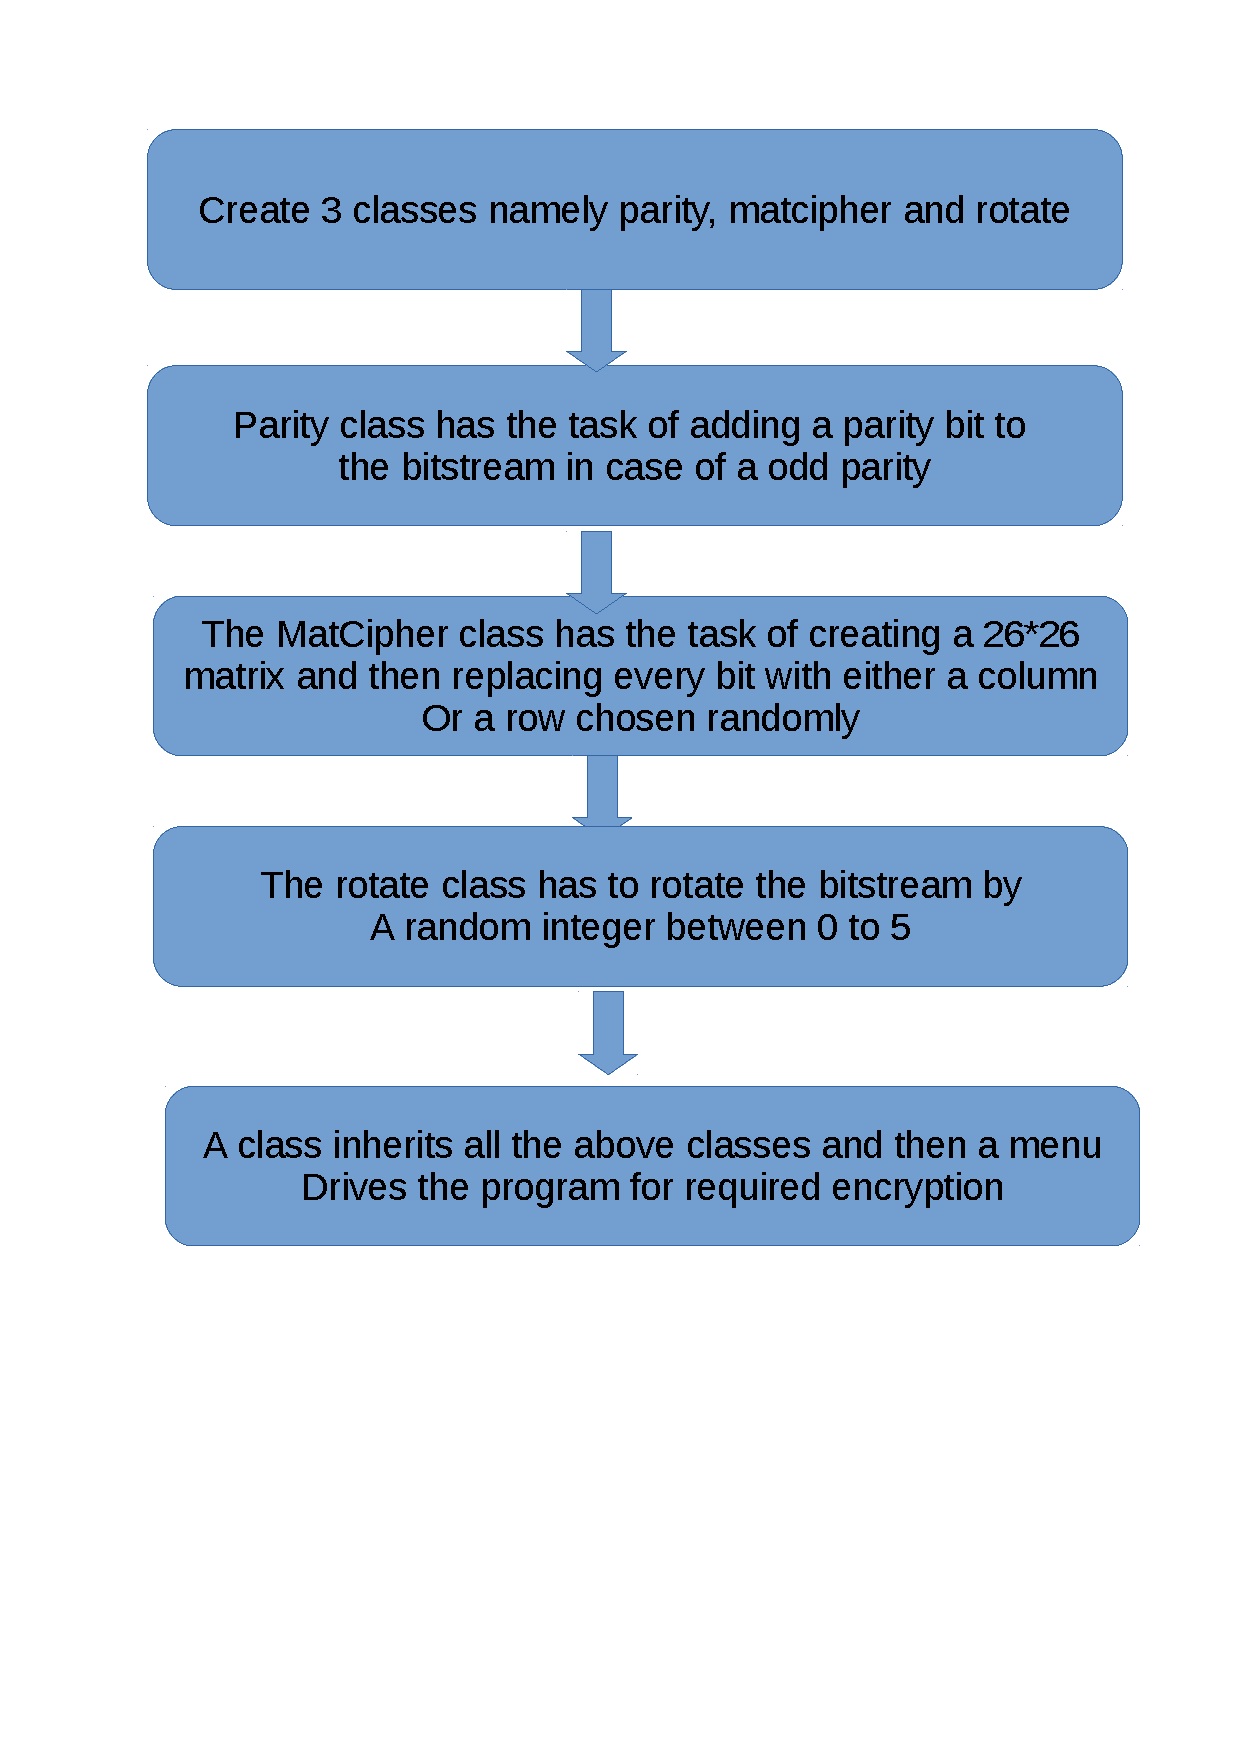
\includegraphics[scale=0.7]{images/shots22}
	\caption{Structure chart for problem 2}	
	\end{figure}
	\pagebreak
	\subsection{Screenshots}
	\begin{figure}[h!]
	\centering
	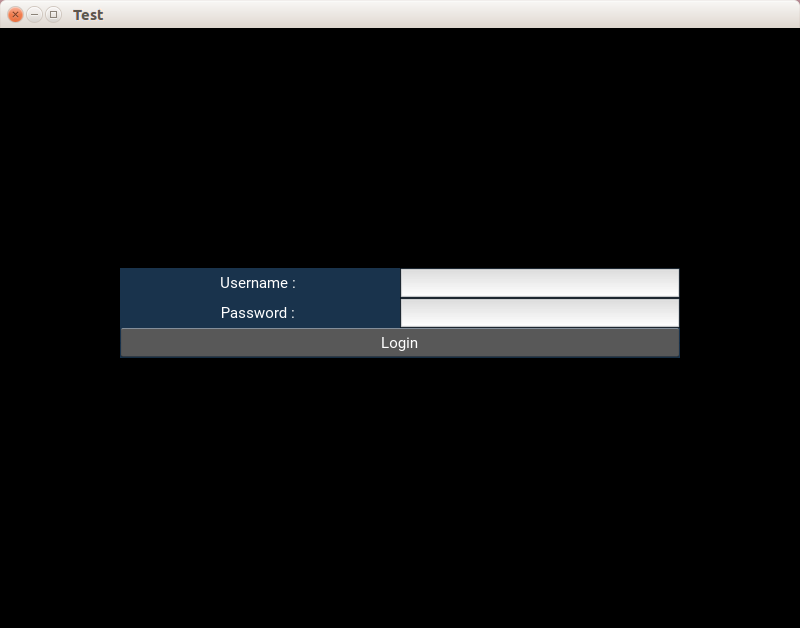
\includegraphics[scale=0.8, center]{images/screenshot2}
	\caption{Screenshot for problem statement 2}
	\end{figure}
	\pagebreak
\section{Problem Statement 3}
\textbf{Part - 1 -}\\
Write shell script to emulate behaviour of bash, but also record every command put up on terminal on a logger.txt file along with time stamp. Your command prompt should look like normal bash command prompt. \\
	\subsection{Assumptions}
	The output is to be processed in the exact manner as shown in the image\\
	\begin{figure}[h!]
	\centering
	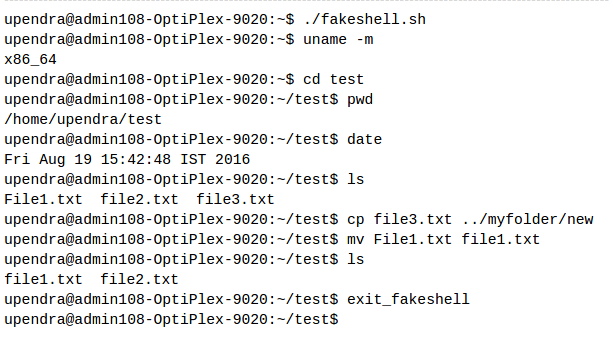
\includegraphics[scale=0.7]{images/Selection_004}	
	\end{figure}
	\pagebreak
	\subsection{Structure Chart}
	\begin{figure}[h!]
	\centering
	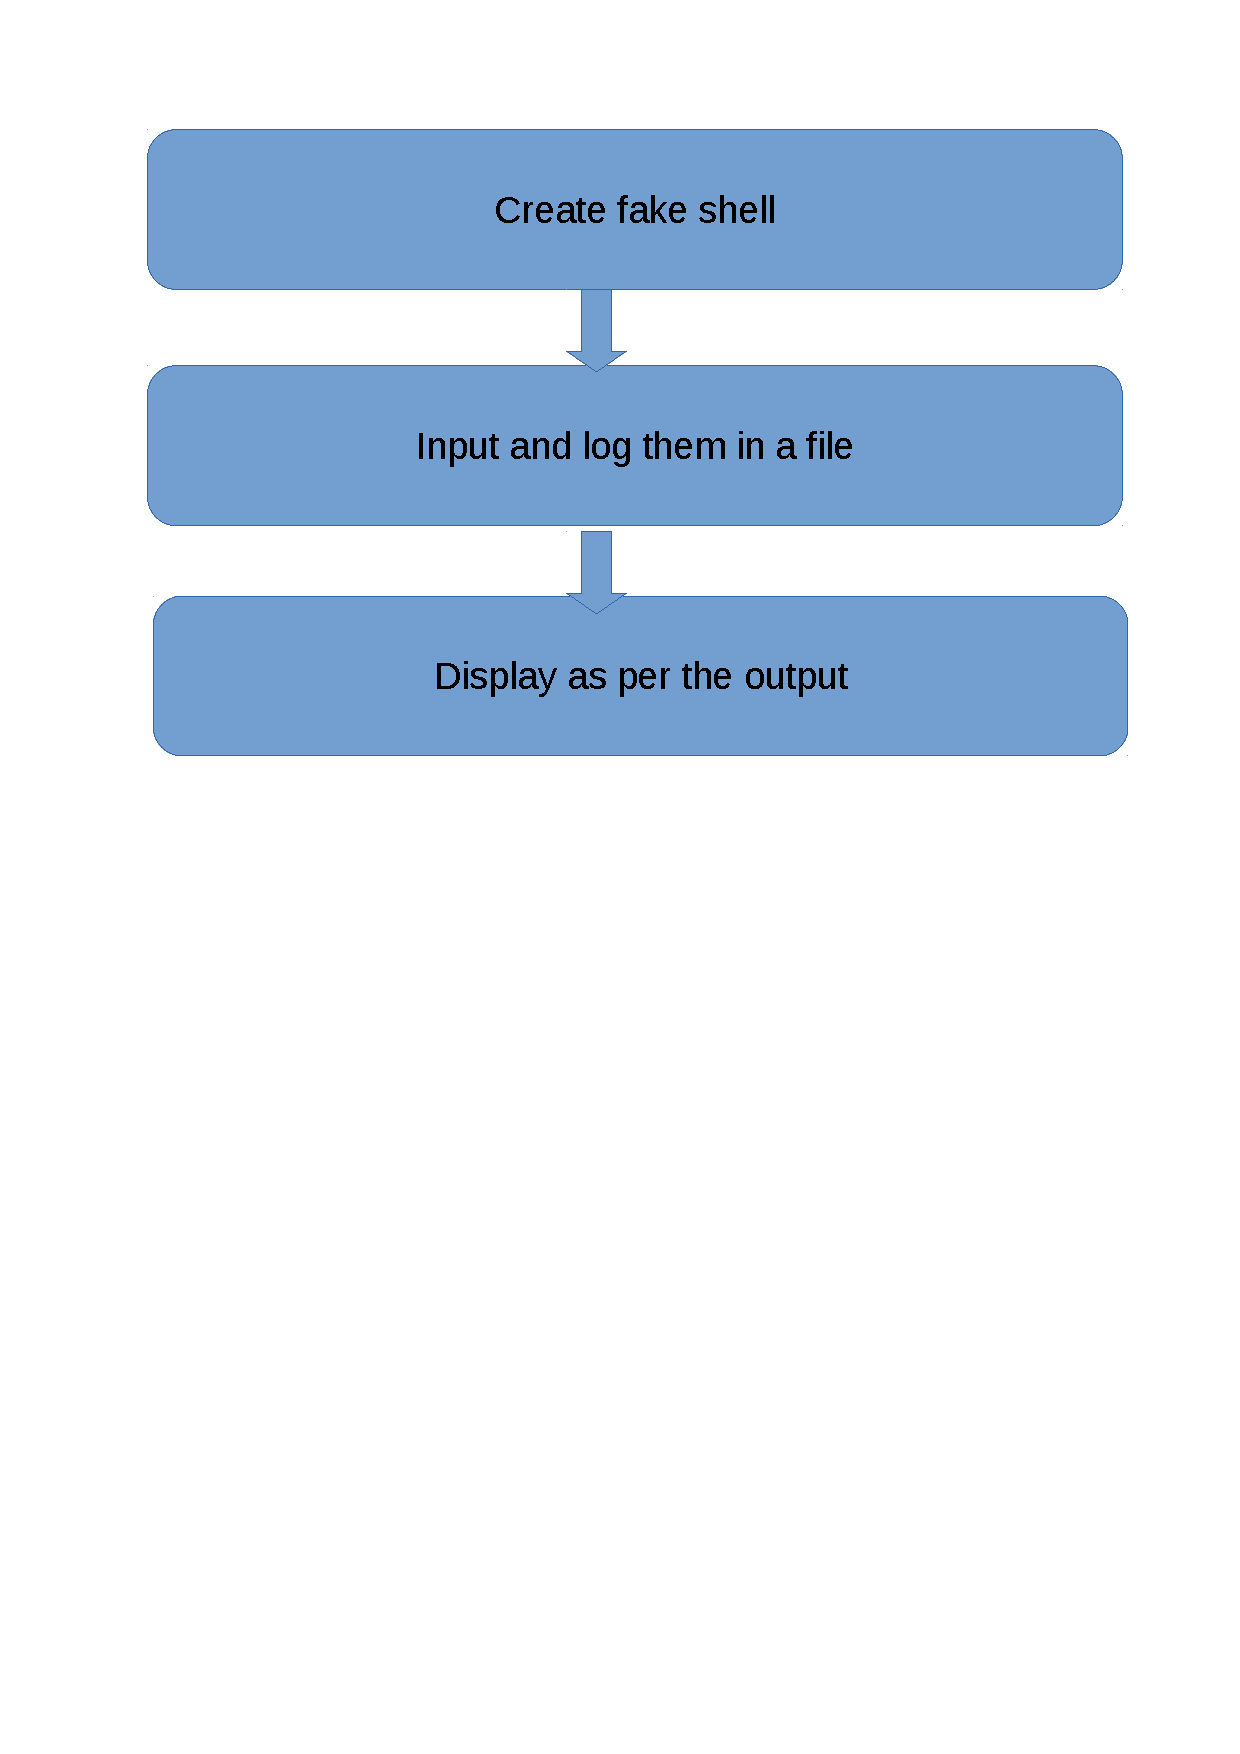
\includegraphics[scale=0.7]{images/shots33}
	\caption{Structure chart for problem 3}	
	\end{figure}
	\pagebreak
\section{Epilogue}
The execution of the first problem involved me to break it down and then try to figure out solution to each and every part of it. To some extent I feel I have been successful in justifying the problem.\\
Whereas for problem statement 2, it was a different but not so difficult problem statement compared to problem 1. \\
Then i found the problem 3 to be the toughest of all problems.\\
This week's assignment too has taught me a lot of things on which I shall further improve upon in the next assignment.\\
\bibliography{biblio} 
\bibliographystyle{ieeetr}
\nocite{*}
\end{document}